\documentclass{article}
\setlength{\parskip}{0pt} % esp. entre parrafos
\setlength{\parindent}{3pt} % esp. al inicio de un parrafo
\usepackage{amsmath} % mates
\usepackage{listings}
\usepackage[sort&compress,numbers]{natbib} % referencias
\usepackage{url} % que las URLs se vean lindos
\usepackage[top=10mm,left=20mm,right=20mm,bottom=25mm]{geometry} % \textbf{\textbf{}}margenes
\usepackage{hyperref} % ligas de URLs
\usepackage{graphicx} % poner figuras
\usepackage[spanish]{babel} % otros idiomas
\hypersetup{
    colorlinks=true,
    linkcolor=blue,
    filecolor=blue,      
    urlcolor=blue,
    citecolor=black,
}

\title{TAREA \# 4 \\ Diagramas de Voronoi} %titulo
\author{Natalia Berenice P\'{e}rez L\'{o}pez} % author
\date{\today}

\begin{document} % inicia contenido

\maketitle % cabecera

\section{Objetivo}
El objetivo de esta práctica es examinar el efecto del número de semillas $k$ en la penetración de las grietas que se forman, en términos de la mayor distancia Manhattan entre la grieta y el borde de la pieza, todo esto manteniendo constante el tamaño $n$ de la zona, visualizando los resultados con diagramas caja-bigote o similar sobre las réplicas y aplicando métodos estadísticos para establecer el efecto de $k$ en ello.

\section{Desarrollo} % seccion y etiqueta
Para generar el código objetivo de esta práctica se realizaron diversos códigos prueba, los cuales se encuentran en \href{https://github.com/nataliaperez0/Simulation/tree/main/Tarea4}{mi repositorio}  en GitHub. Se inició tomando como base el código revisado en clase \citep{1} para generar una matríz de tamaño $n$ que contiene cierta cantidad de semillas $k$ y que es fracturada por una grieta de longitud y dirección aleatoria. Los valores que se elegieron para las variables del experimento se muestran en el cuadro \ref{Cuadro 1}.

\begin{table}[ht]
\centering
\caption{Variables del experimento.}
\smallskip

 \begin{tabular}{ |p{4cm}|p{3cm}|}
 \hline
 VARIABLE & VALOR \\
 \hline
 Semillas ($k$) & $6$, $12$, $24$ \\
 \hline
 Réplicas    & $15$ para cada $k$ \\
 \hline
 Tamaño de la matríz ($n$) & $18$ \\
 \hline
\end{tabular}
\label{Cuadro 1}
\end{table}

Las modificaciones que se le realizaron al código de \texttt{RStudio} revisado en clase fueron; agregar un ciclo \texttt{for} para variar $k$, cambiar el número de réplicas y definir el tamaño constante de la matríz. Se intentó modificar el código para obtener automáticamente la distancia Manhattan de la penetración de la fractura al borde de la matríz, pero esto no resultó con éxito. También se realizó una videollamada con mi compañera Claudia Hernández para discutir ideas sobre como realizar el objetivo de la práctica, sin embargo tampoco tuvimos éxito, por lo cual óptamos por la idea de calcular la distancia Manhattan en \texttt{excel} utilizando las posiciones de los $0$ de la matríz, la cual se puede obtener fácilmente en \texttt{RStudio}. Con las matrices exportadas a \texttt{excel} se realizó el cálculo de las distancias de cada posición a los bordes de la matríz, después se obtuvieron la distancias mínimas y de éstas se obtuvo la distancia máxima que hace referencia a la distancia Manhattan de los bordes a la posición más profunda que tiene la grieta. 

A continuación se muestra un fragmento del código utilizado para varíar el número de semillas $k$.

\definecolor{morado}{rgb}{0.34,0.13,0.39}
\definecolor{codegray}{rgb}{0.5,0.5,0.5}
\definecolor{codegreen}{rgb}{0,0.56,0.22}
\definecolor{backcolour}{rgb}{0.95,0.95,0.92}
\definecolor{azul}{rgb}{0,0,1}

\lstdefinestyle{mystyle}{
    backgroundcolor=\color{backcolour},   
    commentstyle=\color{morado},
    keywordstyle=\color{azul},
    numberstyle=\tiny\color{codegray},
    stringstyle=\color{codegreen},
    basicstyle=\ttfamily\footnotesize,
    breakatwhitespace=false,         
    breaklines=true,                 
    captionpos=b,                    
    keepspaces=true,                 
    numbers=left,                    
    numbersep=5pt,                  
    showspaces=false,                
    showstringspaces=false,
    showtabs=false,                  
    tabsize=2
}
\lstset{style=mystyle}
\begin{lstlisting}[language=R, caption= Código para varíar la cantidad de semillas $k$.]
n <-  18
numsem <- c(6, 12, 24)

for (k in numsem) {
  zona <- matrix(rep(0, n * n), nrow = n, ncol = n)
  x <- rep(0, k) # ocupamos almacenar las coordenadas x de las semillas
  y <- rep(0, k) # igual como las coordenadas y de las semillas
  
  for (semilla in 1:k) {
    while (TRUE) { #hasta que hallamos una posicion vacia para la semilla
      fila <- sample(1:n, 1)
      columna <- sample(1:n, 1)
      if (zona[fila, columna] == 0){
        zona[fila, columna] = semilla
        x[semilla] <- columna
        y[semilla] <- fila
        break
      }
    }
  }
  
  celda <- function(pos){
    fila <- floor((pos - 1) / n) + 1
    columna <- ((pos - 1) %% n) + 1
    if (zona[fila, columna] > 0){ #es una semilla
      return(zona[fila, columna])
    } else{
      cercano <- NULL #sin valor por el momento
      menor <- n * sqrt(2) #mayor posible para comenzar la busqueda
      for (semilla in 1:k){
        dx <- columna - x[semilla]
        dy <- fila - y[semilla]
        dist <- sqrt(dx^2 + dy^2)
        if (dist < menor){
          cercano <- semilla
          menor <- dist
        }
      }
      return(cercano)
    }
  }
  
  celdas <- sapply(1:(n * n), function(p) celda(p))
  voronoi <- matrix(celdas, nrow = n, ncol = n, byrow=TRUE)
  rotate <- function(x) t(apply(x, 2, rev))
  sem=paste("p4s", "-", k, ".png", sep="")
  png(sem)
  par(mar = c(0,0,0,0))
  image(rotate(zona), col=rainbow(k+1), xaxt='n', yaxt='n')
  graphics.off()
  cel=paste("p4c", "-", k, ".png", sep="")
  png(cel)
  par(mar = c(0,0,0,0))
  image(rotate(voronoi), col=rainbow(k+1), xaxt='n', yaxt='n')
  graphics.off()
}

\end{lstlisting}

Enseguida se muestra el fragmento del código que permite exportar a \texttt{excel} la matríz que contiene la fractura. 

\definecolor{morado}{rgb}{0.34,0.13,0.39}
\definecolor{codegray}{rgb}{0.5,0.5,0.5}
\definecolor{codegreen}{rgb}{0,0.56,0.22}
\definecolor{backcolour}{rgb}{0.95,0.95,0.92}
\definecolor{azul}{rgb}{0,0,1}

\lstdefinestyle{mystyle}{
    backgroundcolor=\color{backcolour},   
    commentstyle=\color{morado},
    keywordstyle=\color{azul},
    numberstyle=\tiny\color{codegray},
    stringstyle=\color{codegreen},
    basicstyle=\ttfamily\footnotesize,
    breakatwhitespace=false,         
    breaklines=true,                 
    captionpos=b,                    
    keepspaces=true,                 
    numbers=left,                    
    numbersep=5pt,                  
    showspaces=false,                
    showstringspaces=false,
    showtabs=false,                  
    tabsize=2
}
\lstset{style=mystyle}
\begin{lstlisting}[language=R, caption= Código para exportar la matríz de la fractura a \texttt{excel}.]
    if (elegido > 0) { # si se va a propagar
      vecino <- vp[elegido,]
      xg <- xg + vecino$dx
      yg <- yg + vecino$dy
    } else {
      break # ya no se propaga
    }
  }
  if (largo >= limite) {
    png(paste("p4g_", replica, ".png", sep=""))
    par(mar = c(0,0,0,0))
    image(rotate(grieta), col=rainbow(k+1), xaxt='n', yaxt='n')
    graphics.off()
  }
  return(grieta)
}

suppressMessages(library(doParallel))
registerDoParallel(makeCluster(detectCores() - 1))
lagrieta <- foreach(r = 1:1, .combine=c) %dopar% propaga(r)
stopImplicitCluster()
lagrieta
datos = rbind(datos, lagrieta)
write_xlsx(datos, "misdatos.xlsx")

\end{lstlisting}

\newpage
.
\bigskip

Para cada $0$ que tenía la matríz se obtuvo su coordenada $x, y$ y se calcularon las distancias hacia el borde izquierdo, derecho, superior e inferior de la siguiente manera:

\begin{table}[ht]
\centering
\caption{Fórmulas para calcular las distancias.}
\smallskip

 \begin{tabular}{ |p{5cm}|p{5cm}|}
 \hline
 $di = x$ & distancia al borde izquierdo \\
 \hline
 $dd = n - x$ & distancia al borde derecho \\
 \hline
 $ds = n - y$ & distancia al borde superior \\
 \hline
 $din= y$ & distancia al borde inferior \\
 \hline
 $menores = min(di, dd, ds, din)$ & distancia mínima \\
 \hline
 $max(menores)$ & distancia Manhattan \\
 \hline
\end{tabular}
\label{Cuadro 2}
\end{table}

Las distancias Manhattan que se obtuvieron para cada réplica se muestran en el cuadro \ref{Cuadro 3}.

\begin{table}[ht]
\centering
\caption{Distancias Manhattan de acuerdo a número de semillas para cada réplica.}
\smallskip

 \begin{tabular}{|p{1.5cm}|p{5.5cm}|}
 \hline
 Semillas & Distancias Manhattan \\ \hline
 $6$ & $6$, $4$, $5$, $5$, $9$, $4$, $6$, $7$, $9$, $4$, $9$, $7$, $6$, $5$, $7$
 \\ \hline
 $12$ & $9$, $6$, $4$, $9$, $9$, $4$, $5$, $5$, $5$, $8$, $9$, $5$, $6$, $6$, $4$
 \\ \hline
 $24$ & $9$, $8$, $5$, $9$, $9$, $4$, $6$, $5$, $9$, $9$, $9$, $9$, $8$, $9$, $5$
\\ \hline
\end{tabular}
\label{Cuadro 3}
\end{table}
\bigskip

Las distancias del cuadro 3 se importaron de \texttt{excel} a \texttt{RStudio} para realizar el diagrama caja-bigote mostrado en la figura \ref{Figura 1}.

\begin{figure} [h!]% figura
    \centering
    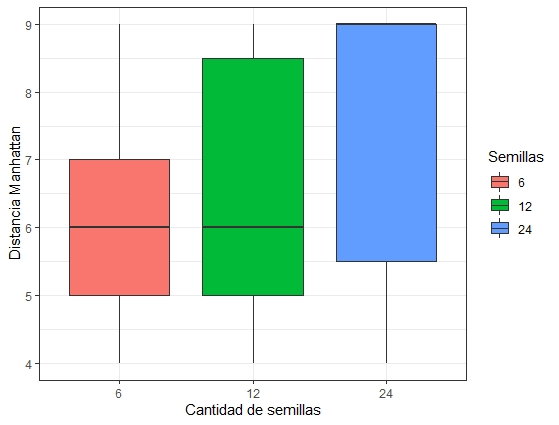
\includegraphics[width=130mm]{Figura1.jpeg} % archivo
    \caption{Distancia Manhattan de acuerdo al número de semillas en una matríz de $n = 18$.}
    \label{Figura 1}
\end{figure}

En la figura \ref{Figura 1} podemos observar que con un número pequeño de semillas se obtienen distancias más cortas para la penetración de la fractura, y al aumentar el número de semillas la distancia de penetración de la fracutra se puede hacer más larga.

\newpage
.
\bigskip

Para analizar si existe una relación entre la variación del número de semillas y la distancia de penetración de la fractura, primero se elegió utilizar la prueba estadística ANOVA de una vía, pero debido a los resultados obtenidos al revisar la normalidad de los datos, se eligió realizar la prueba estadística \texttt{Kruskal Wallis} \citep{2}.
\bigskip

En el cuadro \ref{Cuadro 4} se  resumen los resultados de la revisión de los supuestos para poder aplicar la prueba estadística ANOVA. El supuesto outliers se refiere a la cantidad de valores atípicos que existen en los grupos, la normalidad por grupos se obtuvo con la prueba de \texttt{Shapiro Wilk}, y la homogeneidad de varianza se obtuvo con la prueba de \texttt{Levene}.

\begin{table}[ht]
\centering
\caption{Resultados del los supuestos para aplicar la prueba estadística ANOVA.}
\smallskip

\begin{tabular}{ |p{2.1cm}|p{3.5cm}|}
 \hline
 Outliers & $0$ \\
 \hline
 Normalidad por grupo & 6 semillas: $p$ = $0.0749$ 12 semillas: $p$ = $0.0100$ 24 semillas: $p$ = $0.0006$ \\
 \hline
 Homogeneidad de varianza & $p$ = $0.926$ \\
 \hline
\end{tabular}
\label{Cuadro 4}
\end{table}

En los resultados se observa que los datos de los grupos de 12 y 24 semillas no tienen normalidad. Por lo tanto se debe realizar la prueba estadística \texttt{Kruskal Wallis} ya que ésta es útil para cuando no se tiene normalidad en los grupos de datos.
\bigskip

Al realizar la prueba \texttt{Kruskal Wallis} se obtienen los resultados mostrados en el cuadro 5.

\begin{table}[ht]
\centering
\caption{Resultados al aplicar la prueba estadística \texttt{Kruskal Wallis}.}
\smallskip

\begin{tabular}{ |p{2.1cm}|p{2.1cm}|}
 \hline
 Chi cuadrada & Valor de $p$ \\
 \hline
 $3.8803$ & $0.1437$ \\
 \hline
\end{tabular}
\label{Cuadro 5}
\end{table}

Hipótesis nula : Las medias son iguales en todos los grupos
\smallskip

Debido a que $p > 0.05$ se acepta la hipótesis nula, no existen diferencias significativas entre las medias de los grupos. Se entiende entonces que la variación de las semillas $k$ no tiene un efecto significativo en la distancia de la penetración de la fractura. 
\bigskip

A continuación se muestra el código para realizar las pruebas estadísticas:

\definecolor{morado}{rgb}{0.34,0.13,0.39}
\definecolor{codegray}{rgb}{0.5,0.5,0.5}
\definecolor{codegreen}{rgb}{0,0.56,0.22}
\definecolor{backcolour}{rgb}{0.95,0.95,0.92}
\definecolor{azul}{rgb}{0,0,1}

\lstdefinestyle{mystyle}{
    backgroundcolor=\color{backcolour},   
    commentstyle=\color{morado},
    keywordstyle=\color{azul},
    numberstyle=\tiny\color{codegray},
    stringstyle=\color{codegreen},
    basicstyle=\ttfamily\footnotesize,
    breakatwhitespace=false,         
    breaklines=true,                 
    captionpos=b,                    
    keepspaces=true,                 
    numbers=left,                    
    numbersep=5pt,                  
    showspaces=false,                
    showstringspaces=false,
    showtabs=false,                  
    tabsize=2
}
\lstset{style=mystyle}
\begin{lstlisting}[language=R, caption= Código para hacer la prueba estadística Kruskal Wallis.]
#PRUEBA ESTADISTICA
library(readxl)
library(ggplot2)
library(tidyverse)
library(ggpubr)
library(car)

ruta_excel = "C:\\Users\\beren\\OneDrive\\Escritorio\\Maestría\\2do semestre\\5. Simulación computacional de nanomateriales\\Tareas\\Tarea_4\\datos.xlsx"
datos = read_excel(ruta_excel)
datos

datos$Semillas= as.factor(datos$Semillas) #crear vector a partir del dataframe

diagrama = ggplot(data = datos, aes(x = Semillas, y = Distancia, fill = Semillas)) +
  geom_boxplot() + theme_bw() + labs(x = "Cantidad de semillas", y = "Distancia Manhattan")

diagrama

#Estadisticas descriptivas
datos = datos %>%
  rstatix::reorder_levels(Semillas, order = c("6", "12", "24"))

datos %>%
  group_by(Semillas) %>%
  get_summary_stats(Distancia, type = "mean_sd")

#SUPUESTOS PARA ANOVA
#1:Outliers
datos %>%
  group_by(Semillas) %>%
  identify_outliers(Distancia)

#2:Normalidad con residuales
normalidad = lm(Distancia ~ Semillas, data = datos)
head(datos)
head(normalidad$fitted.values)
head(normalidad$residuals)

grafica1 = ggqqplot(residuals(normalidad))+
  labs(title = 'Normalidad con residuales')
grafica1

shapiro_test(residuals(normalidad))

datos %>%
  group_by(Semillas) %>%
  shapiro_test(Distancia)

#3:Homogeneidad de varianza con prueba Levene
datos %>%
  levene_test(Distancia~Semillas)


#PRUEBA ESTADISTICA KRUSKAL WALLIS
kruskal.test(Distancia ~ Semillas, data = datos)

pairwise.wilcox.test(datos$Distancia, datos$Semillas)

grafica2 = ggline(data = datos, x = "Semillas", y = "Distancia", add = c("mean_se", "jitter"))
grafica2
  
\end{lstlisting}

\newpage
.
\bigskip

\section{Conclusi\'{o}n}
Con base en los resultados obtenidos de la prueba estadística \texttt{Kruskal Wallis} puedo concluir que el hecho de variar la cantidad de semillas en la matríz no influye tanto en la distancia de la penetración de la grieta, sin embargo en el diagrama caja-bigote se puede observar que cuando existen más semillas la distancia puede tener valores más grandes pero no deja de presentar valores pequeños al igual que con pocas semillas. 
\smallskip

En general ésta práctica me permitió darme cuenta que me falta mejorar en el entendimiento de los códigos para ser capaz de modificarlos de manera adecuada, también me permitió aplicar otras pruebas estadísticas y analizar su utilidad.
\newpage
.
\bigskip

\bibliography{referencias}
\bibliographystyle{plainnat}

\end{document}